\section{Implementation}


\subsection{Data models}

A dataset definition for clinical research will consist of a number of
different parts, each of which declares a set of related data items.
Typically, this will be a set of data items that would be collected
together: in the completion of a `case report form' in a study, or in
the report of a clinical event.  These parts may be `repeating', in
that there may be more than one form of that type completed, or more
than one event of that type reported upon.  

A data item declaration should explain not only the name under which
values are to be stored, but also the type of those values.  If the
type is numeric, then the unit of measurement should be given.  If the
type is an enumeration, then the intended interpretation of each value
should be explained.  Finally, the parts of the dataset may be
connected or related to one another, and these relationships may have
constrained multiplicities.

It should be clear that a dataset definition can be represented as a
class diagram or object model.  Data items can be introduced as
attributes, parts of the model as classes, and relationships between
classes as associations---complete with multiplicities.  Data types
and enumerations can be used to support attribute declarations, and
hence data item definitions; constraints can be used to express range
restrictions and intended relationships between data items.

Class diagrams can be used also to provide precise definitions for
data sources: existing clinical systems or research databases.  These
systems may be implemented using a combination of technologies but,
assuming that the value of the data justifies the effort required,
precise object models can be created to describe the interfaces that
they might present for data re-use. 

\subsection{Models as metadata}

Having constructed precise object models to describe datasets and data
sources, we can use them as a basis for automated software and data
engineering.  This involves the use of models as metadata in three
respects: for software artefacts that are generated or configured; for
data that these artefacts store or process; and for other models,
capturing relationships between data points declared in different
models, and hence the data stored or processed against them.

For the first of these, we need only maintain the relationship between
the implementation and the model that was used to generate or
configure it.  If the model is stored in a repository or \emph{model
  catalogue} and published, then we have only to create a link between
the implementation and this published instance.  This link may be
created automatically in the case where the model is generated,
partially or completely, from an existing implementation: for example,
from the schema of a relational database.

For the second, a link must be created between each data point, or
collection of data points, and the corresponding declaration in the
data model.  The model catalogue then requires some support for the
language in which the data model is expressed, sufficient to support
the creation and manipulation of links to specific components: in
particular, to specific classes and attributes.  If the data is
acquired or processed using a software implementation for which a data
model has already been registered, then that model may provide a basis
for the automatic creation of a link to the corresponding declaration.

For the third, we need the same ability to create and manipulate links
between components of different models.  Instead of links between
model and implementation, however, we have links representing
different kinds of relationships: provenance and re-use of model
components; versioning of models; and, most importantly,
\emph{semantic relationships} between attributes or
classes---assertions that one attribute or class has the same meaning
or interpretation as another.  This is precisely the information
needed to support automation in data discovery, integration, and
re-use.

\subsection{Data Model Language}

The core features of our modelling language are familiar: classes,
associations, attributes, constraints, enumerations, data types.
However, our interpretation of these features is narrower than that
set out in, for example, the specifications of the Unified Modeling
Language (UML)~\cite{UML} or Ecore~\cite{ECORE}.  For this reason, and
because of the need to refer explicitly to models and capture semantic
relationships between models, classes, and attributes, we define a
domain specific language for data models.

We extend this language to include additional modelling features
pertaining to certain kinds of implementation artefacts, such as
forms, messages, databases, and documentation.  This is necessary only
when the feature in question may have a bearing upon the data
semantics, and may thus serve as a source or target for a link
describing a property or relationship.  

For example, a section of a form, corresponding to one or more classes
of data, might comprise information about allergies.  We may wish to
link this section to a term in an ontology recording this fact.  This
makes it easier for someone interested in models of allergy
information to locate and possibly re-use the definitions; it also
adds context to any semantic links to data classes and attributes
associated with that section.

The generated or configured part of an implementation may include
features not described by the data model.  This will be the case
wherever a model-driven or generative approach has been adopted in the
development of an application.  In this case, the artefact generated
from or represented by the data model is itself a model, in a
different modelling language.  The use of a data model, in our domain
specific language, as metadata for this other model should come as no
surprise: it is no different from the use of a model as metadata for
program source code. 

The Models Catalogue, like many software developments, evolved from a mix of requirements on a number of different projects.  Initially a metadata registry was built using an XML database, however problems were encountered with scalability.  Most of the language and metamodel developments were carried out using XText and the Eclipse Modelling Framework, resulting in a usable java code base, however usability requirements neccessitated the refactoring of this software using a stack consisting of Grails and Angular JS. 

Grails is built on the Spring framework, which is not only proven to be very robust and scalable, but is also relatively easy to implement and so enables quick agile development cycles. Previous implementations using Java/Spring and Java/Roo have proved very time-consuming to experiment with, whereas Grails has proven to be more flexible and easier to experiment with.  Domain specific languages (DSL’s) can be  built on this framework, and this capability offered scope to build a DSL based on the LEM DSL specification and meta-model expanded in the previous section.
 
The front end user interface was implemented using a combination of HTML with Javascript and CSS, the principal framework used being Angular JS. Communication with the client was carried out using a REST controller, enabling a variety of clients potentially to link up with the Model Catalogue.

GORM was used as a persistence mechanism, with a MySQL relational database as storage, although different GORM adapters made it possible to attach NO SQL datastores such as Neo4J and MongoDB. The full architectural stack is shown in figure\ref{fig:ApplicationArchitectMDR}

\begin{figure}[here]
	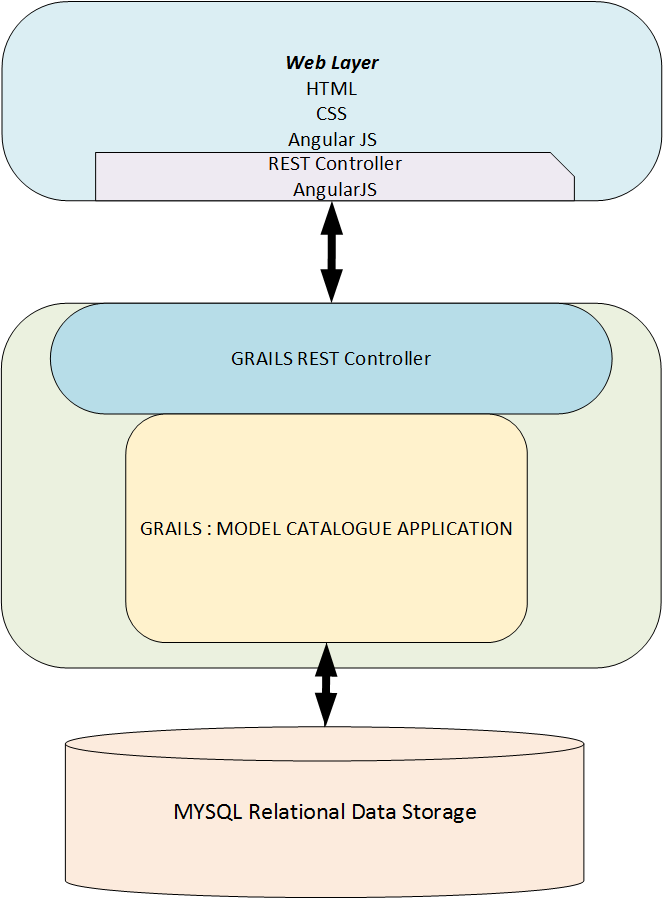
\includegraphics[width=0.48\textwidth,natwidth=610,natheight=642]{ApplicationArchitect1}
	\caption{Overview Architecture} 
	\label{fig:ApplicationArchitectMDR}
\end{figure}

The Grails/GORM framework enabled the Ecore model to generate the basic Grails Domain model, and from that a Groovy DSL was built, using the Builder pattern, to handle transformations internally between different representational languages such as XML and Excel. A series of importers was built for data input from Excel, CSV, and various XML variants. Most XML structures are handled by transforming the XML from its native structure to our internal DSL-based XML structure. 

The internal domain model used a basic \emph{Catalogue Element} which was able to link elements via the \emph{relationship} and \emph{relationshipType} classes. The core language model discussed earlier has been enhanced to by allowing user-defined relationships to be added to the core model. Any catalogue element is able to be related to any other catalogue element through a relationship class, this relationship is constrained by the relationshipType object which can prevent different catalogue element types being related, so that a Model cannot directly be related to a say a Datatype Enumeration. Relationship types can be added to the Model dynamically, so that even though the relationship between a Model and Datatype enumeration is prevented initially, a new type could be introduced by an administrator or super user to add in that relationship. The EMF-based tools to automatically generate the whole Models Catalogue code-base using Groovy/Grails/Angular were not available at the start of the project, and although work has been undertaken to build such a toolkit it not yet complete.  

The following subsections describe the basic use cases for the Model Catalogue, and how these use cases were implemented. 
\subsection{Listing of DataModels}
The key use case required in both projects was the ability to catalogue a set of data elements and data classes so that different schema could be compared and curated. Listing is currently carried out using a REST interface which is queried using an Angular client. Figure \ref{fig:treeviewOfDataModel}
\begin{figure}[here]
	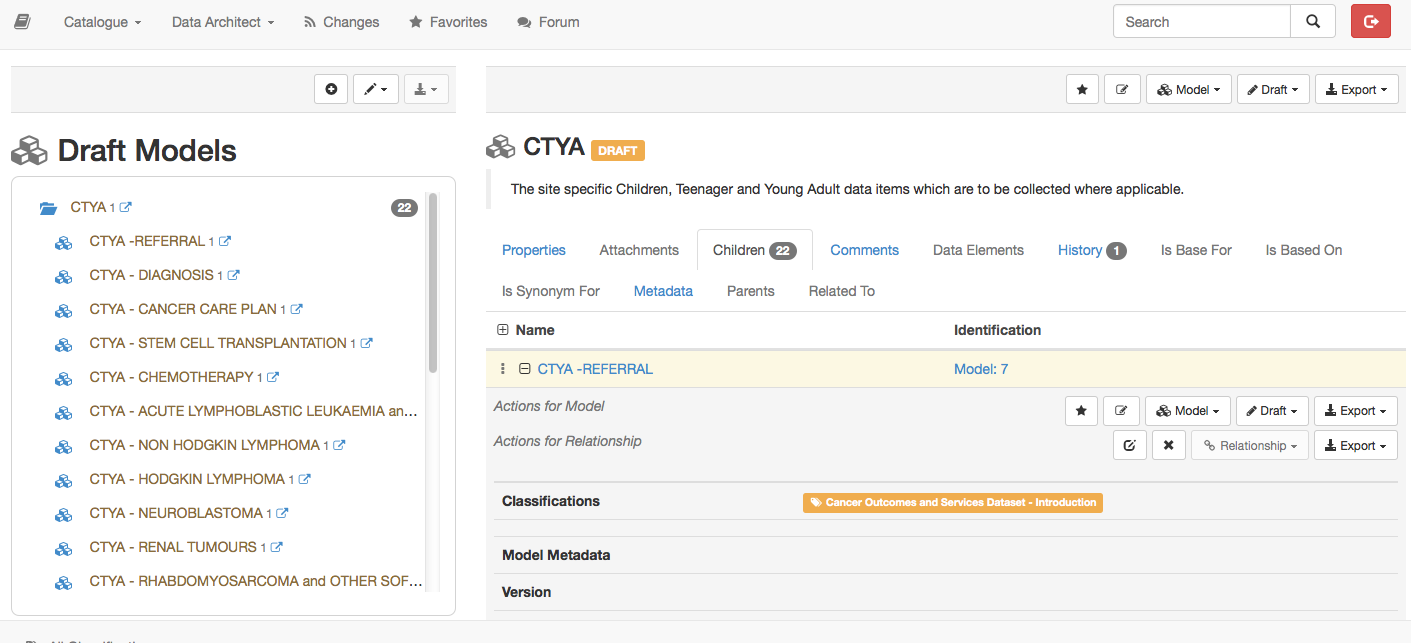
\includegraphics[width=0.5\textwidth,natwidth=610,natheight=642]{DataModelTreeView}
	\caption{Screen Shot of DataModel Listing} 
	\label{fig:treeviewOfDataModel}	
\end{figure}

\subsection{forms}

Typically the initial data models are entity-centric: for example
cancer models are initally built around the entities of
\emph{Patient}, \emph{Tumour}, etc.  Forms are typically structured around
events: \emph{Registration}, \emph{Surgery}, etc.  We construct
separate models for forms, re-using the elements from the
entity-centric model, thus providing a different view upon the same
data.  (As as aside, the Patient Pathway models interact with these
forms models, providing a workflow, ordering form completion).

With respect to forms, we take an approach analagous to that of the
Model-Driven Architecture~\cite{MDA-proposal}: that of
Platform-Specific Models (PSMs) and Platform-Independent models
(PIMs).  Our platform-independent model in this regard is based on the
emerging ISO standard for forms~\cite{ISOForms}.  This provides
structure in terms of \emph{sections}, \emph{sub-sections},
\emph{repeating groups}, and so on, but is not specific to any
particular implementation.  The model is based on previous work on
domain-specific languages for forms~\cite{Abler2011}.

Our initial platform-specific target is \emph{OpenClinica}, a tool for
supporting data capture for clinical trials.  OpenClinica forms are
created using a model supplied in Excel Spreadsheet format.

Our generation of XML schema may also be seen as a platform-specific
implementation of the forms model.  XML schema are used to define
message structures, and have a similar structure to the OpenClinica
forms, although typically additional data is required in XML schema -
context such as the patient for which the data is about, or the person
submitting the data; or linking information which may be automatically
created during manual input into a web interface. 


\subsection{selection of data elements for form generation}
For many clinical users one of the key requirement was the ability to generate forms for clinical research which were generated form a single authorative source, and the ability to take data elements, manage them to build a form and then output either a form or an XML representation for use in another system, such as OpenClinica was key to the work carried out. 



\subsection{relationships between 2 DataModels}
Very often different research groups will arrive at slightly different models for the same or very similar diseased, so another use case for the Models Catalogue was the ability to compare different Data Models, Data Classes and individual Data Elements.






%%-------------------------------
%%Drop next section
%%------------------------------
%%Some of the main relationships that are currently modelled in the \emph{Models Catalogue} are as follows:
 %%
%%\begin{center}
%%	\begin{tabular}{ p{1.5cm}  p{1.5cm}  p{1.5cm}   }  % centered columns (5 columns)
%%		Source & Relationship & Destination  \\
%%		Model & containment & DataElement   \\
%%	    Model & containment & Class    \\
%%	    Model & hierarchical & Model  \\
%%	    DataElement & supersession & DataElement  \\          
%%	\end{tabular}
%%\end{center}
%%
%%The Core architecture can seen in figure\ref{fig:ApplicationArchitectMDR} 
%%
%%\begin{figure}[here]
%%	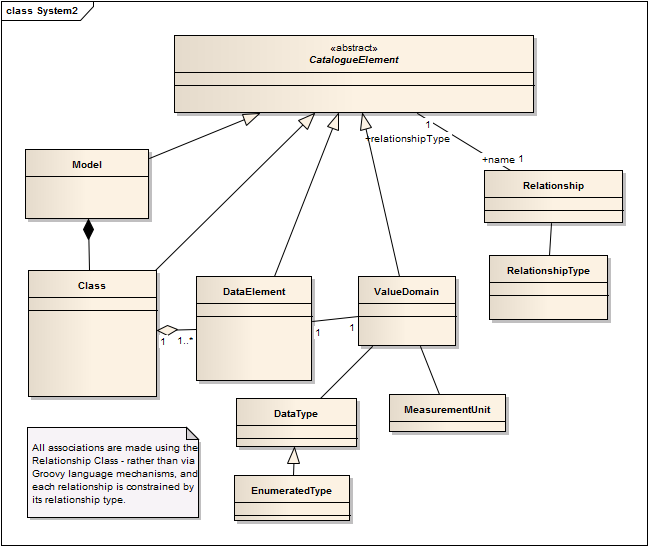
\includegraphics[width=0.5\textwidth,natwidth=610,natheight=642]{System2}
%%	\caption{Overview Architecture} 
%%	\label{fig:System2MDR}
%%\end{figure}
%% 
\subsection{Modelling Overview}





 
 